\subsection{Acceptance Correction}
The largest correction factor in this work is the acceptance correction, which is a convolution of detector efficiency, geometrical acceptance, reconstruction efficiency, and PID and event cuts. We defined acceptance in \eqref{eq:acceptance} as

    \begin{equation*}
      \recallLabel{eq:acceptance},
    \end{equation*}

where we utilize simulations to arrive at an estimator for the acceptance, $\hat{\epsilon}$. The correction term is calculated bin-by-bin, procedurally illustrated in \figref{fig:acccorr}. $\hat{\epsilon}$ values for this analysis were typically on the 1-10\% level. Low acceptance bins were excluded at a threshold of below 0.5\%. The distribution of acceptance correction factors is shown in \figref{fig:acccorrdist}.

    \begin{figure}[H]
        \centering
    
        \subfloat[Raw counts $N_{exp}$.]{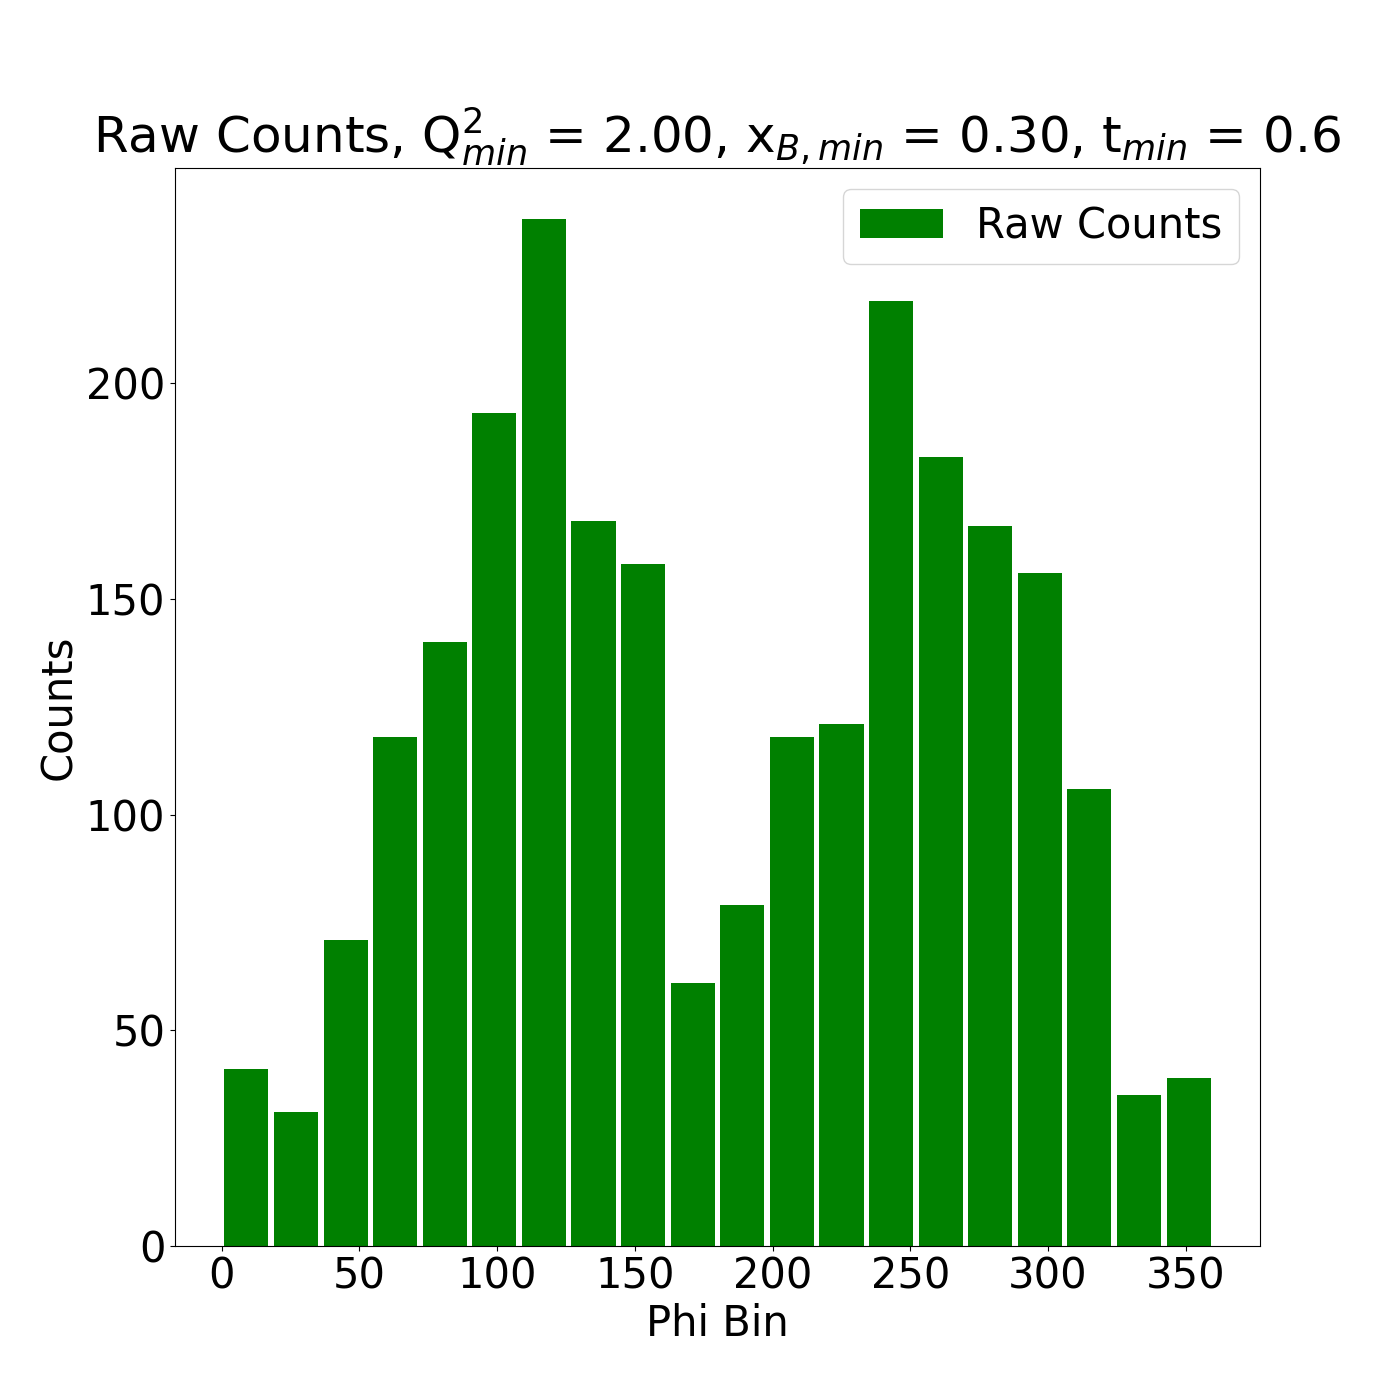
\includegraphics[width=0.5\textwidth]{Chapters/Ch4-BaseAnalysis/4_Correction_Factors/A3_a_acceptance_correction/pics/raw4.png}}
        \hfill
        \subfloat[$N_{gen}$ and $N_{rec}$.]{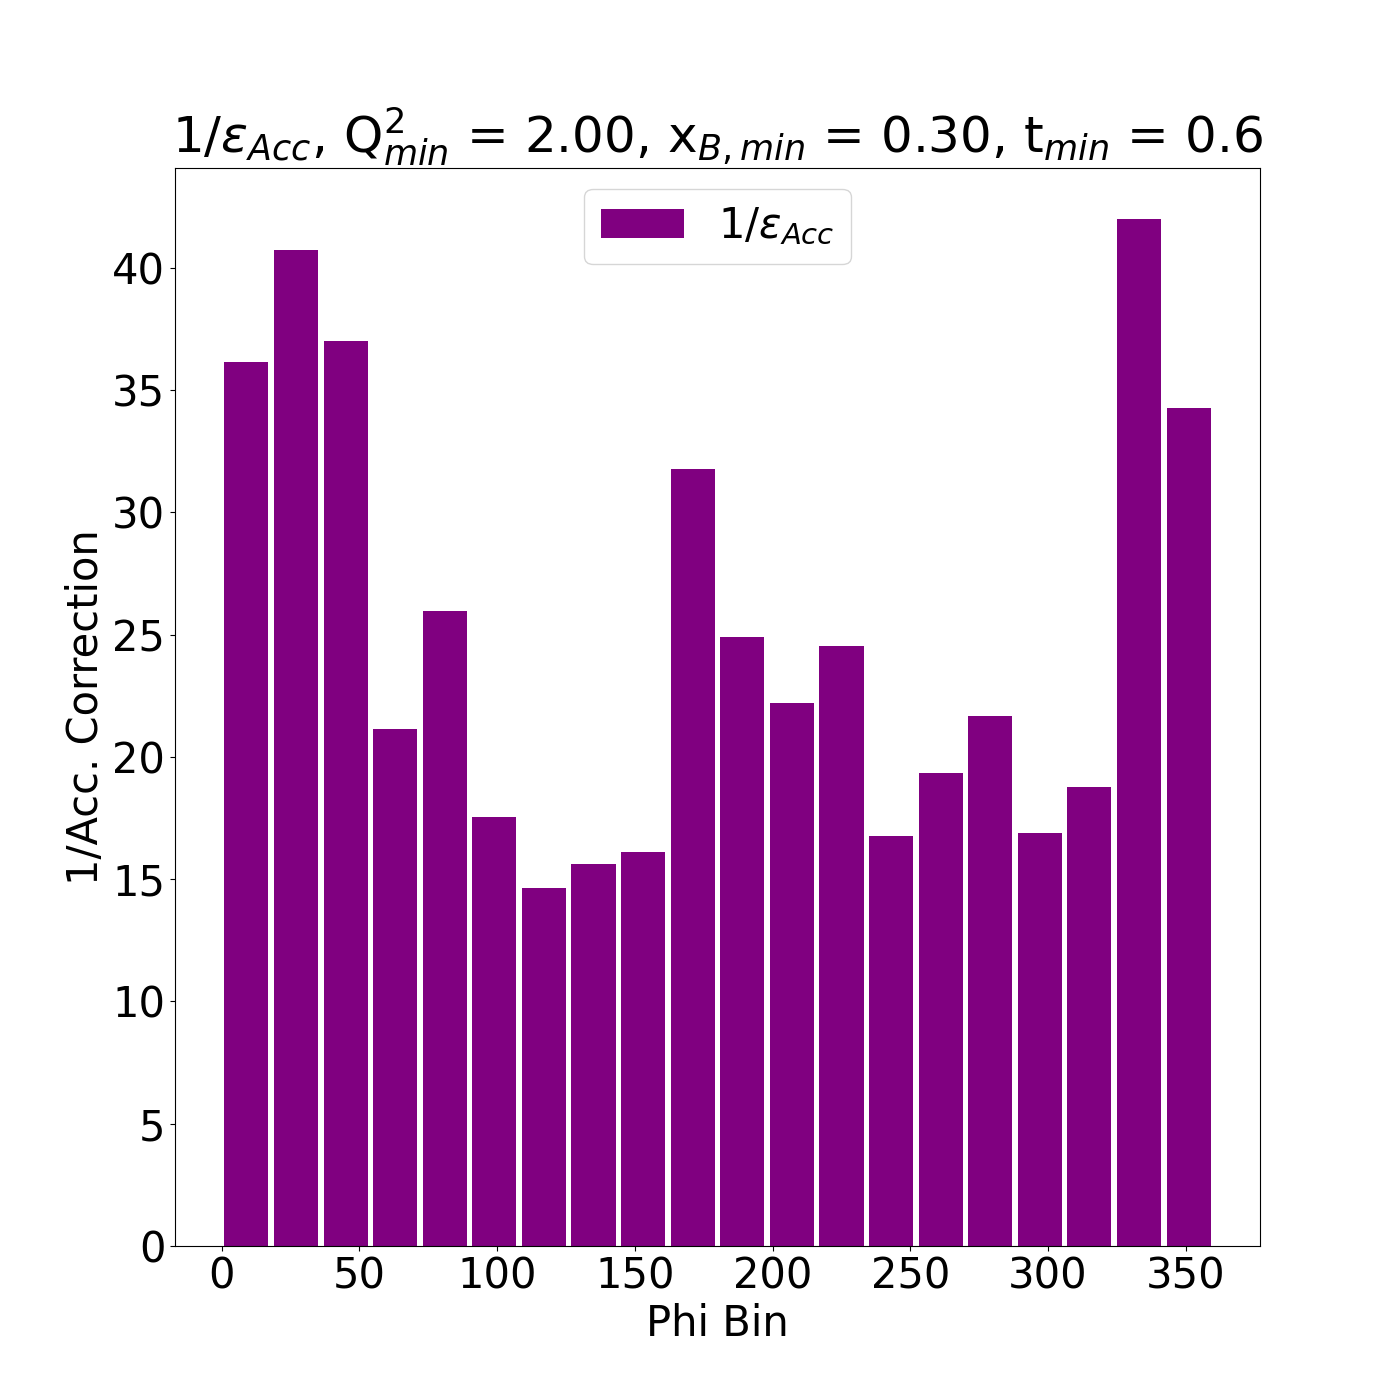
\includegraphics[width=0.5\textwidth]{Chapters/Ch4-BaseAnalysis/4_Correction_Factors/A3_a_acceptance_correction/pics/acc_3.png }}
    
        \subfloat[1/$\hat{\epsilon}$ = $N_{gen}$/$N_{rec}$.]{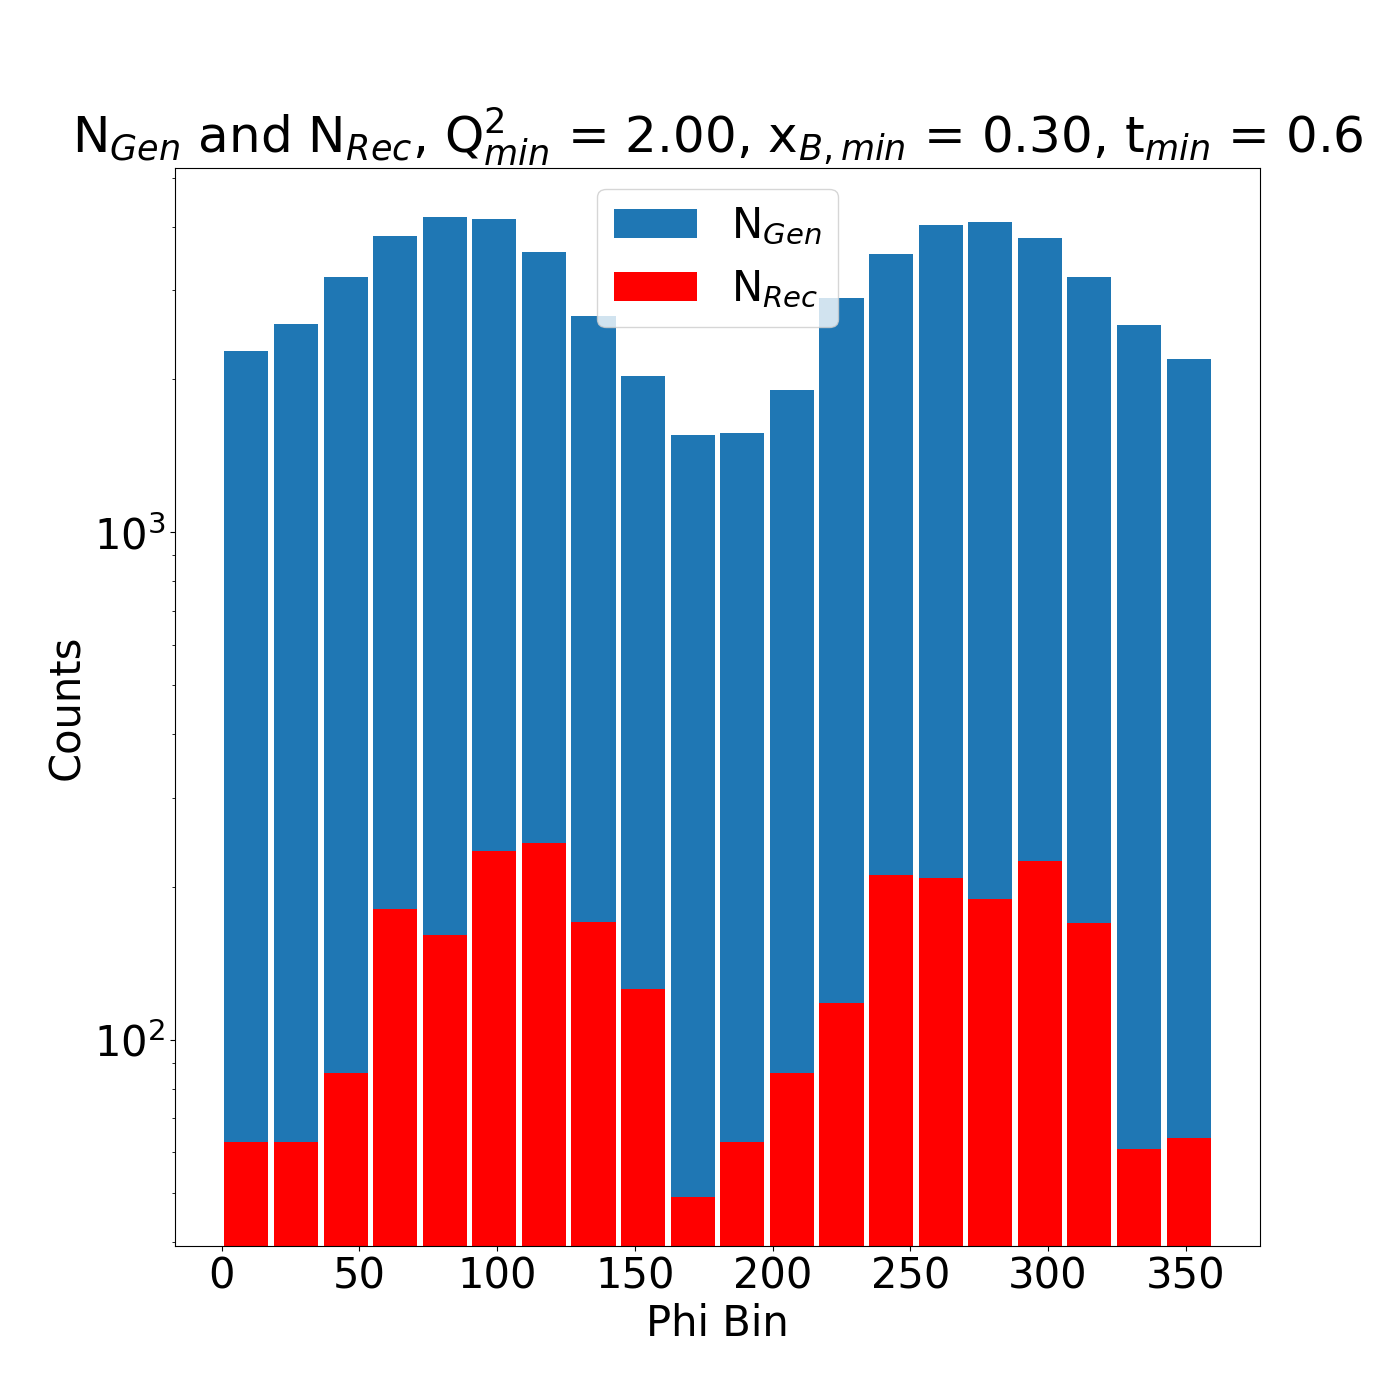
\includegraphics[width=0.5\textwidth]{Chapters/Ch4-BaseAnalysis/4_Correction_Factors/A3_a_acceptance_correction/pics/acc4.png}}
        \hfill
        \subfloat[Acc. Corr Counts = $N_{exp}*N_{gen} / N_{rec}$ ]{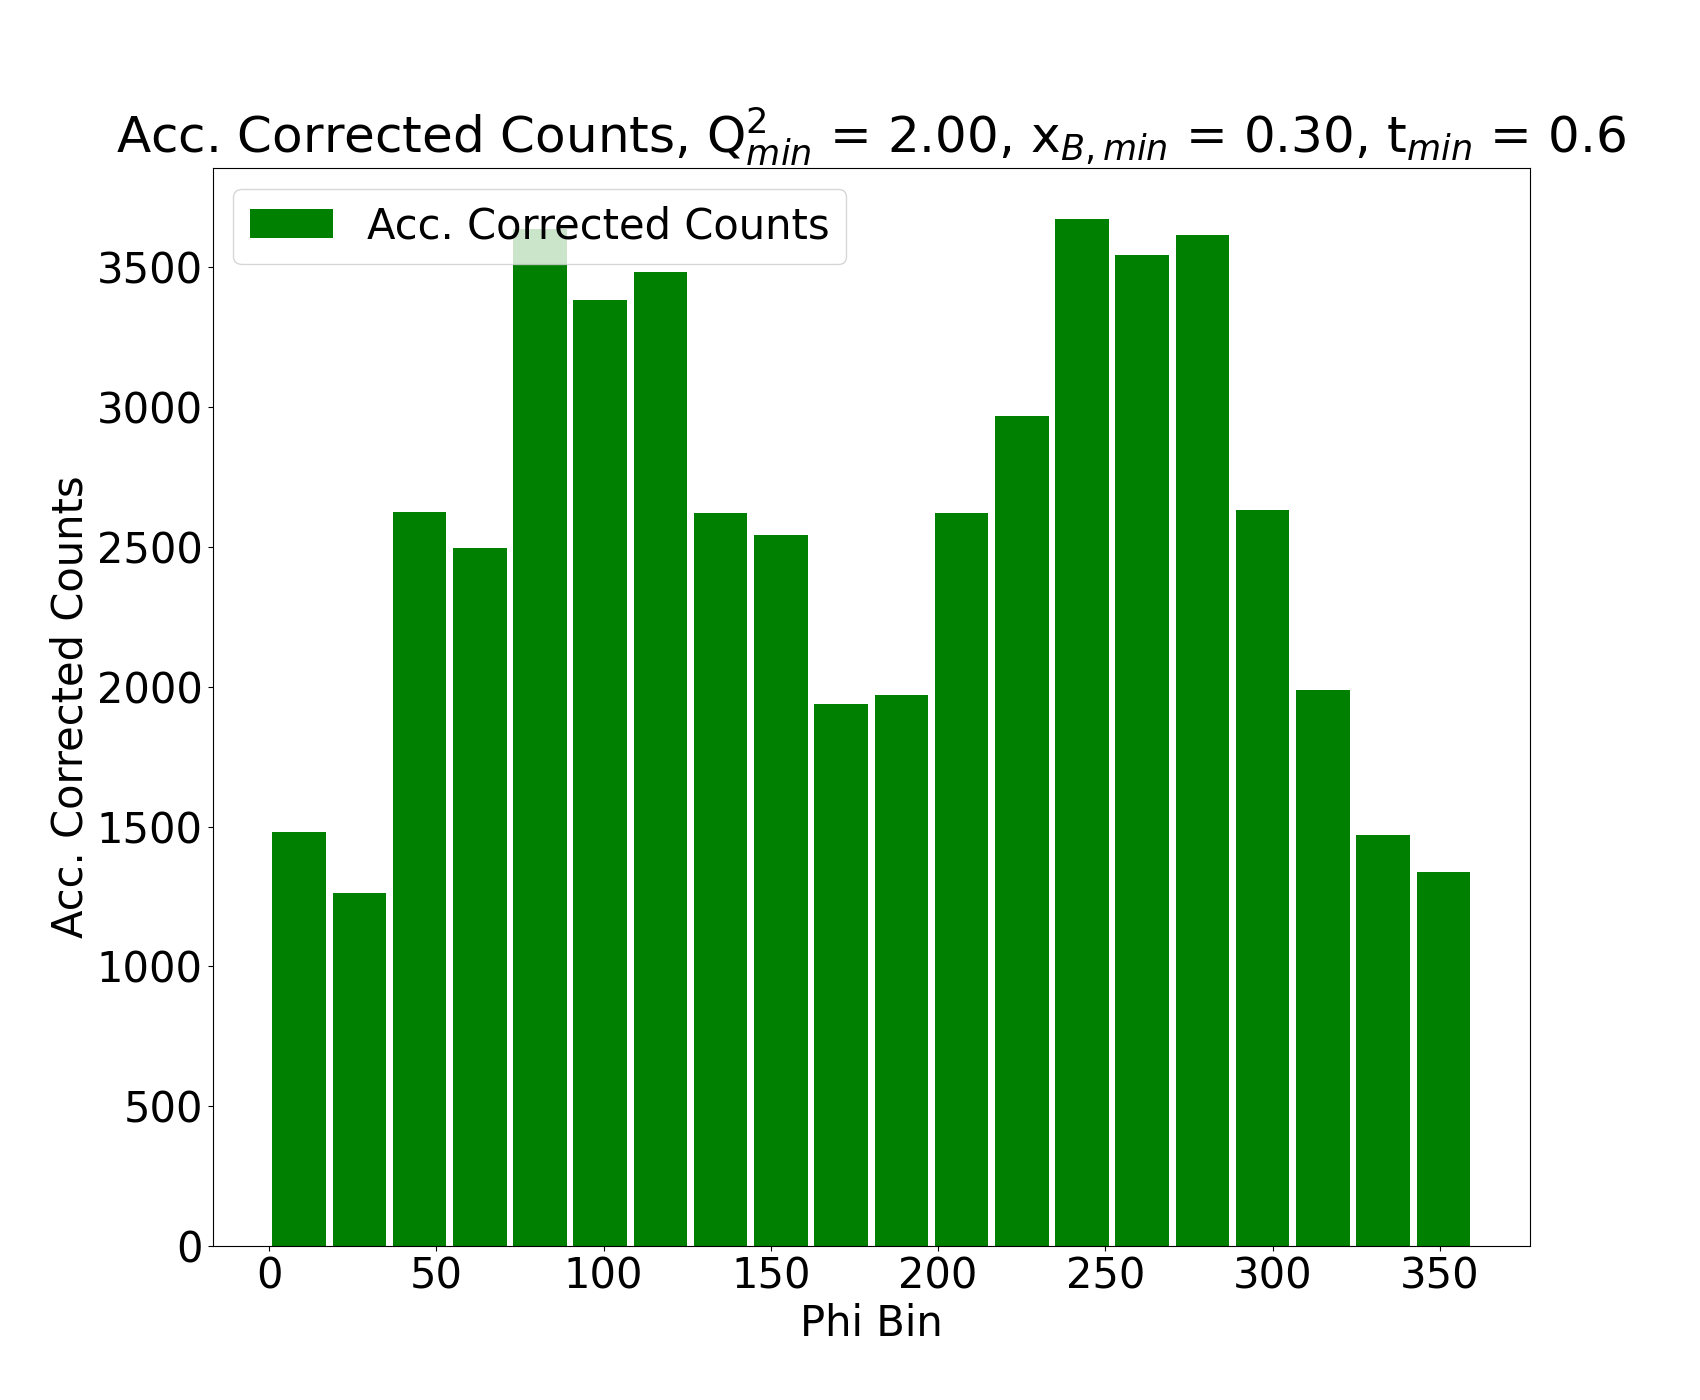
\includegraphics[width=0.5\textwidth]{Chapters/Ch4-BaseAnalysis/4_Correction_Factors/A3_a_acceptance_correction/pics/final2.png}}
    
        \caption[Acceptance Correction Scheme]{Acceptance correction scheme. Experimental events (a), generated and simulated events (b) are all binned, and the ratio of reconstructed simulated events to generated events (c) is multiplied for each $N_{exp}$ to arrive at the acceptance corrected counts (d).}\label{fig:acccorr}
    %\caption[Reduced Cross Sections Across $\phi$]{Reduced Cross Sections Across $\phi$}
\end{figure}



\begin{figure}
    \centering
    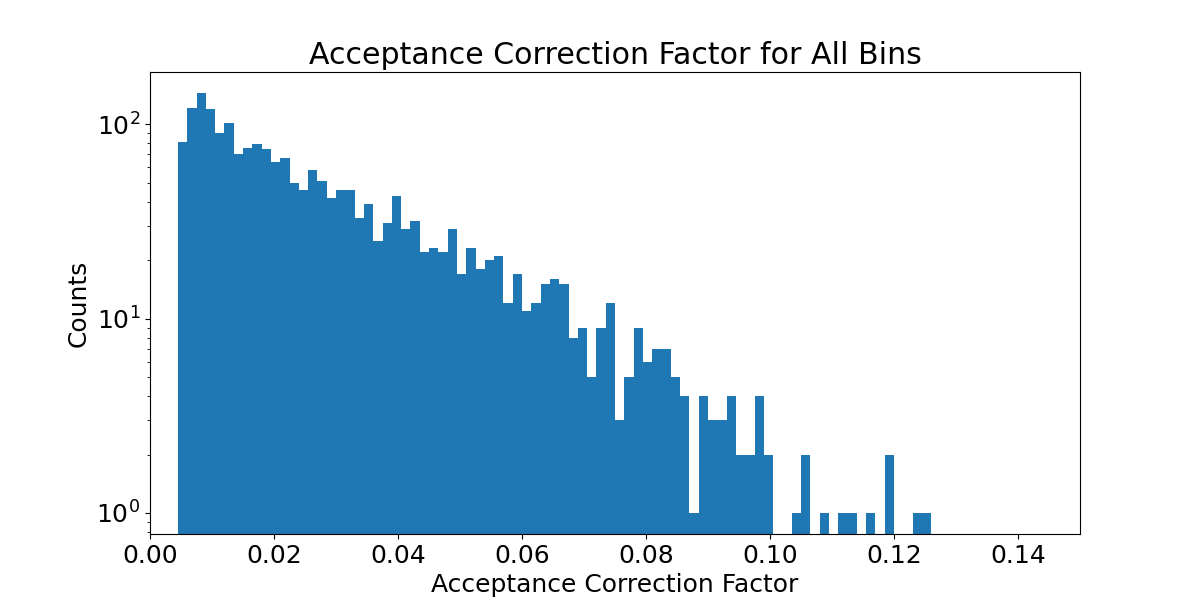
\includegraphics[width=\textwidth]{Chapters/Ch4-BaseAnalysis/4_Correction_Factors/A3_a_acceptance_correction/pics/acccorr.png}
    \caption{Acceptance correction term for all bins.}
    \label{fig:acccorrdist}
\end{figure}




\subsection{Other Corrections}

    \subsubsection*{Radiative Corrections}

    Radiative corrections were estimated using simulations as described in Chapter 3. In particular, the ratio of the acceptance correction between using radiative and non-radiative generated events was taken. Sample results are shown in \figref{fig:radcorr}. 
    
    \begin{figure}[H]
    \centering

    \subfloat[]{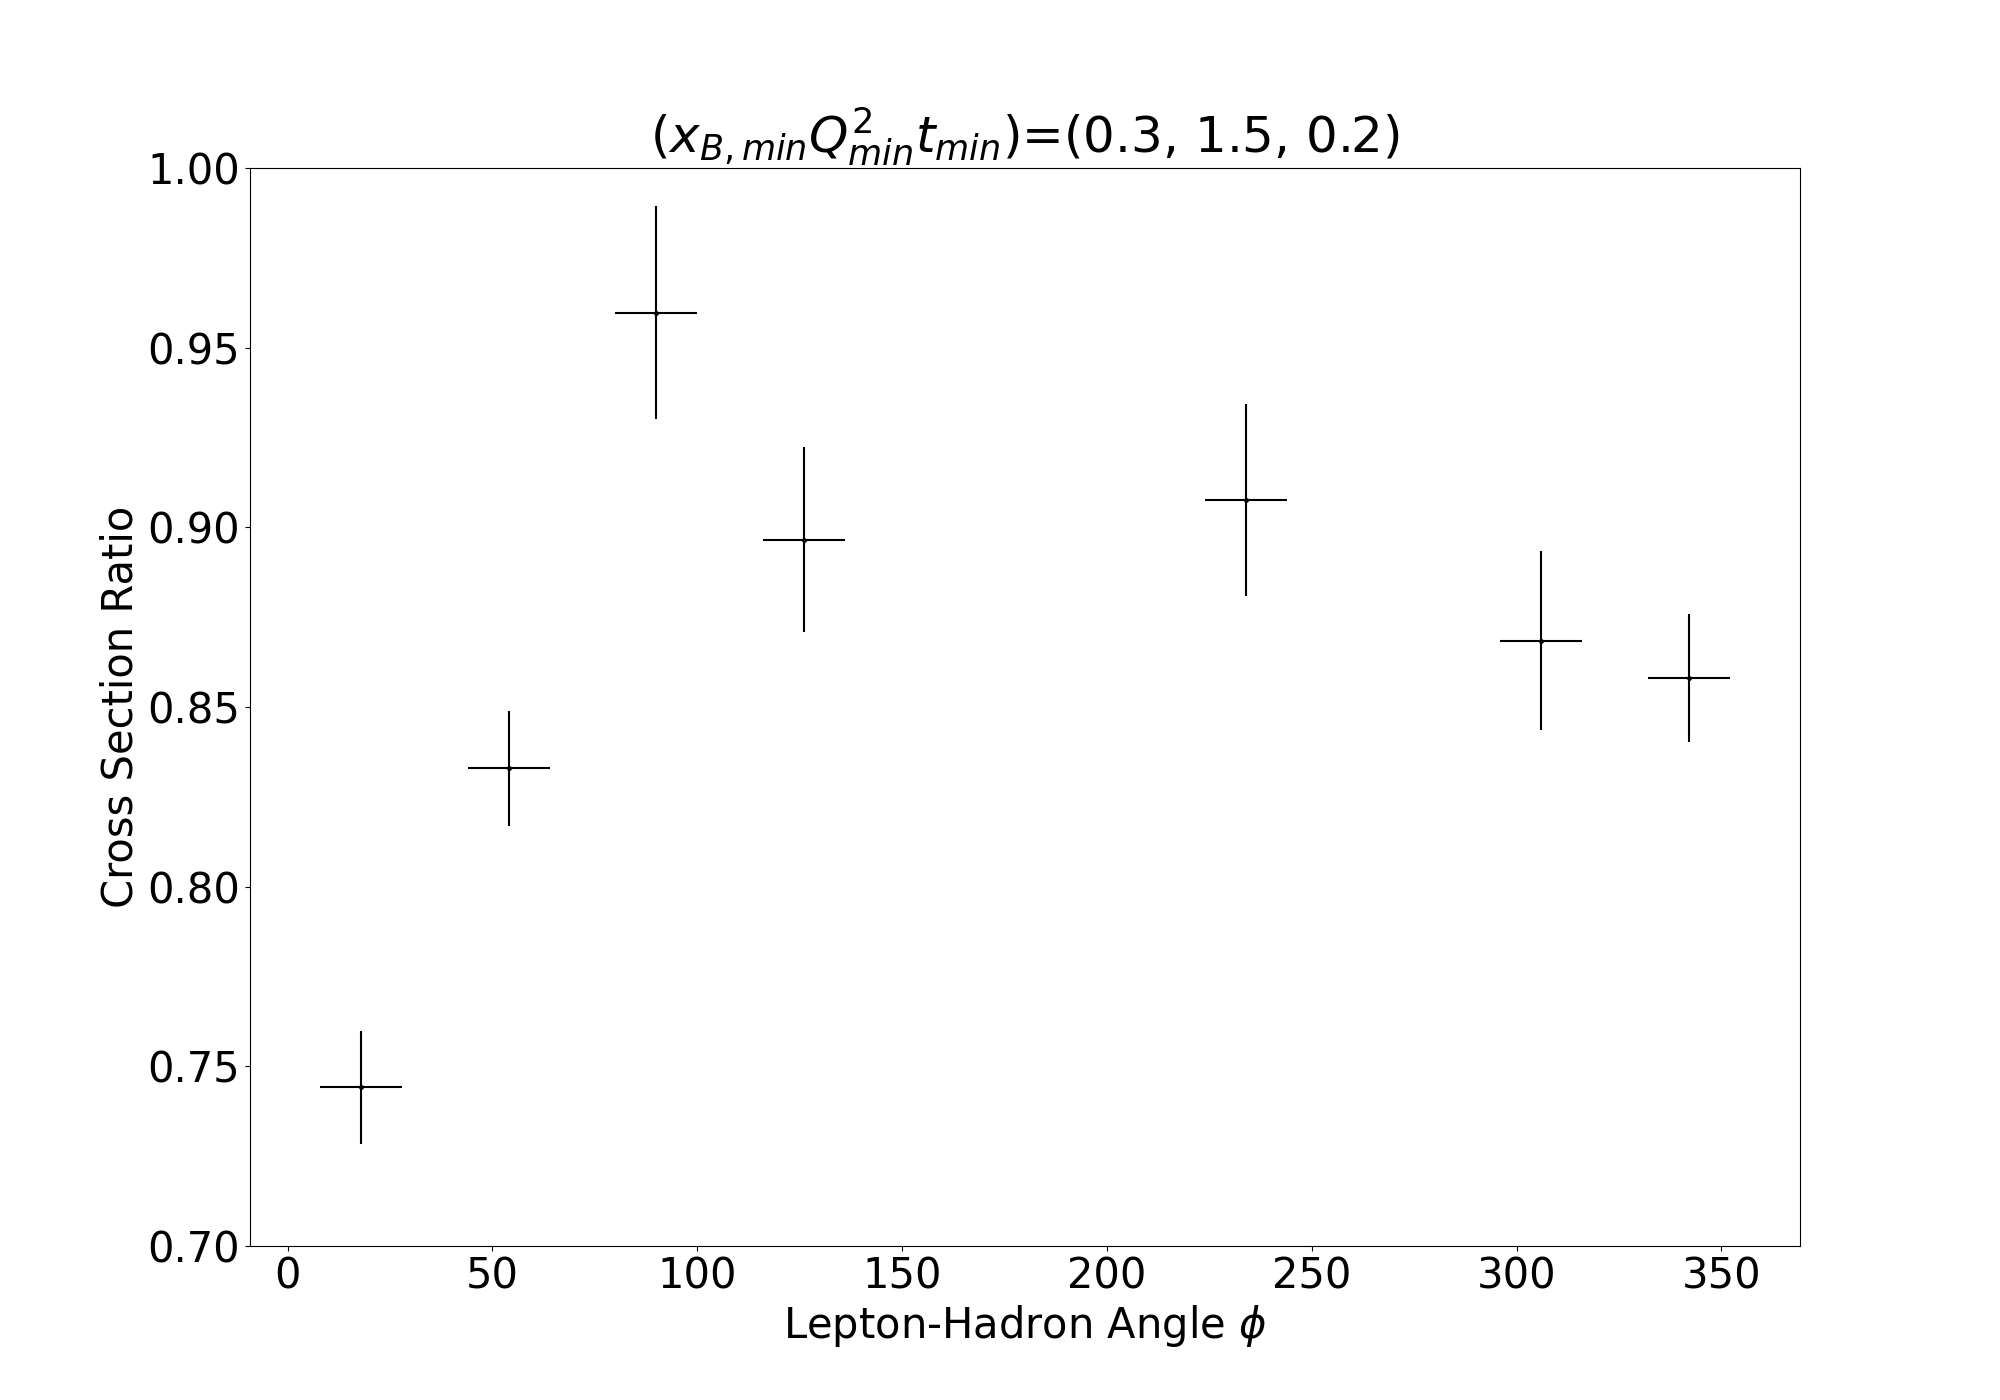
\includegraphics[width=0.5\textwidth]{Chapters/Ch4-BaseAnalysis/4_Correction_Factors/A3_b_radiative_correction/xqt=(0.3, 1.5, 0.2).png}}
    \hfill
    \subfloat[]{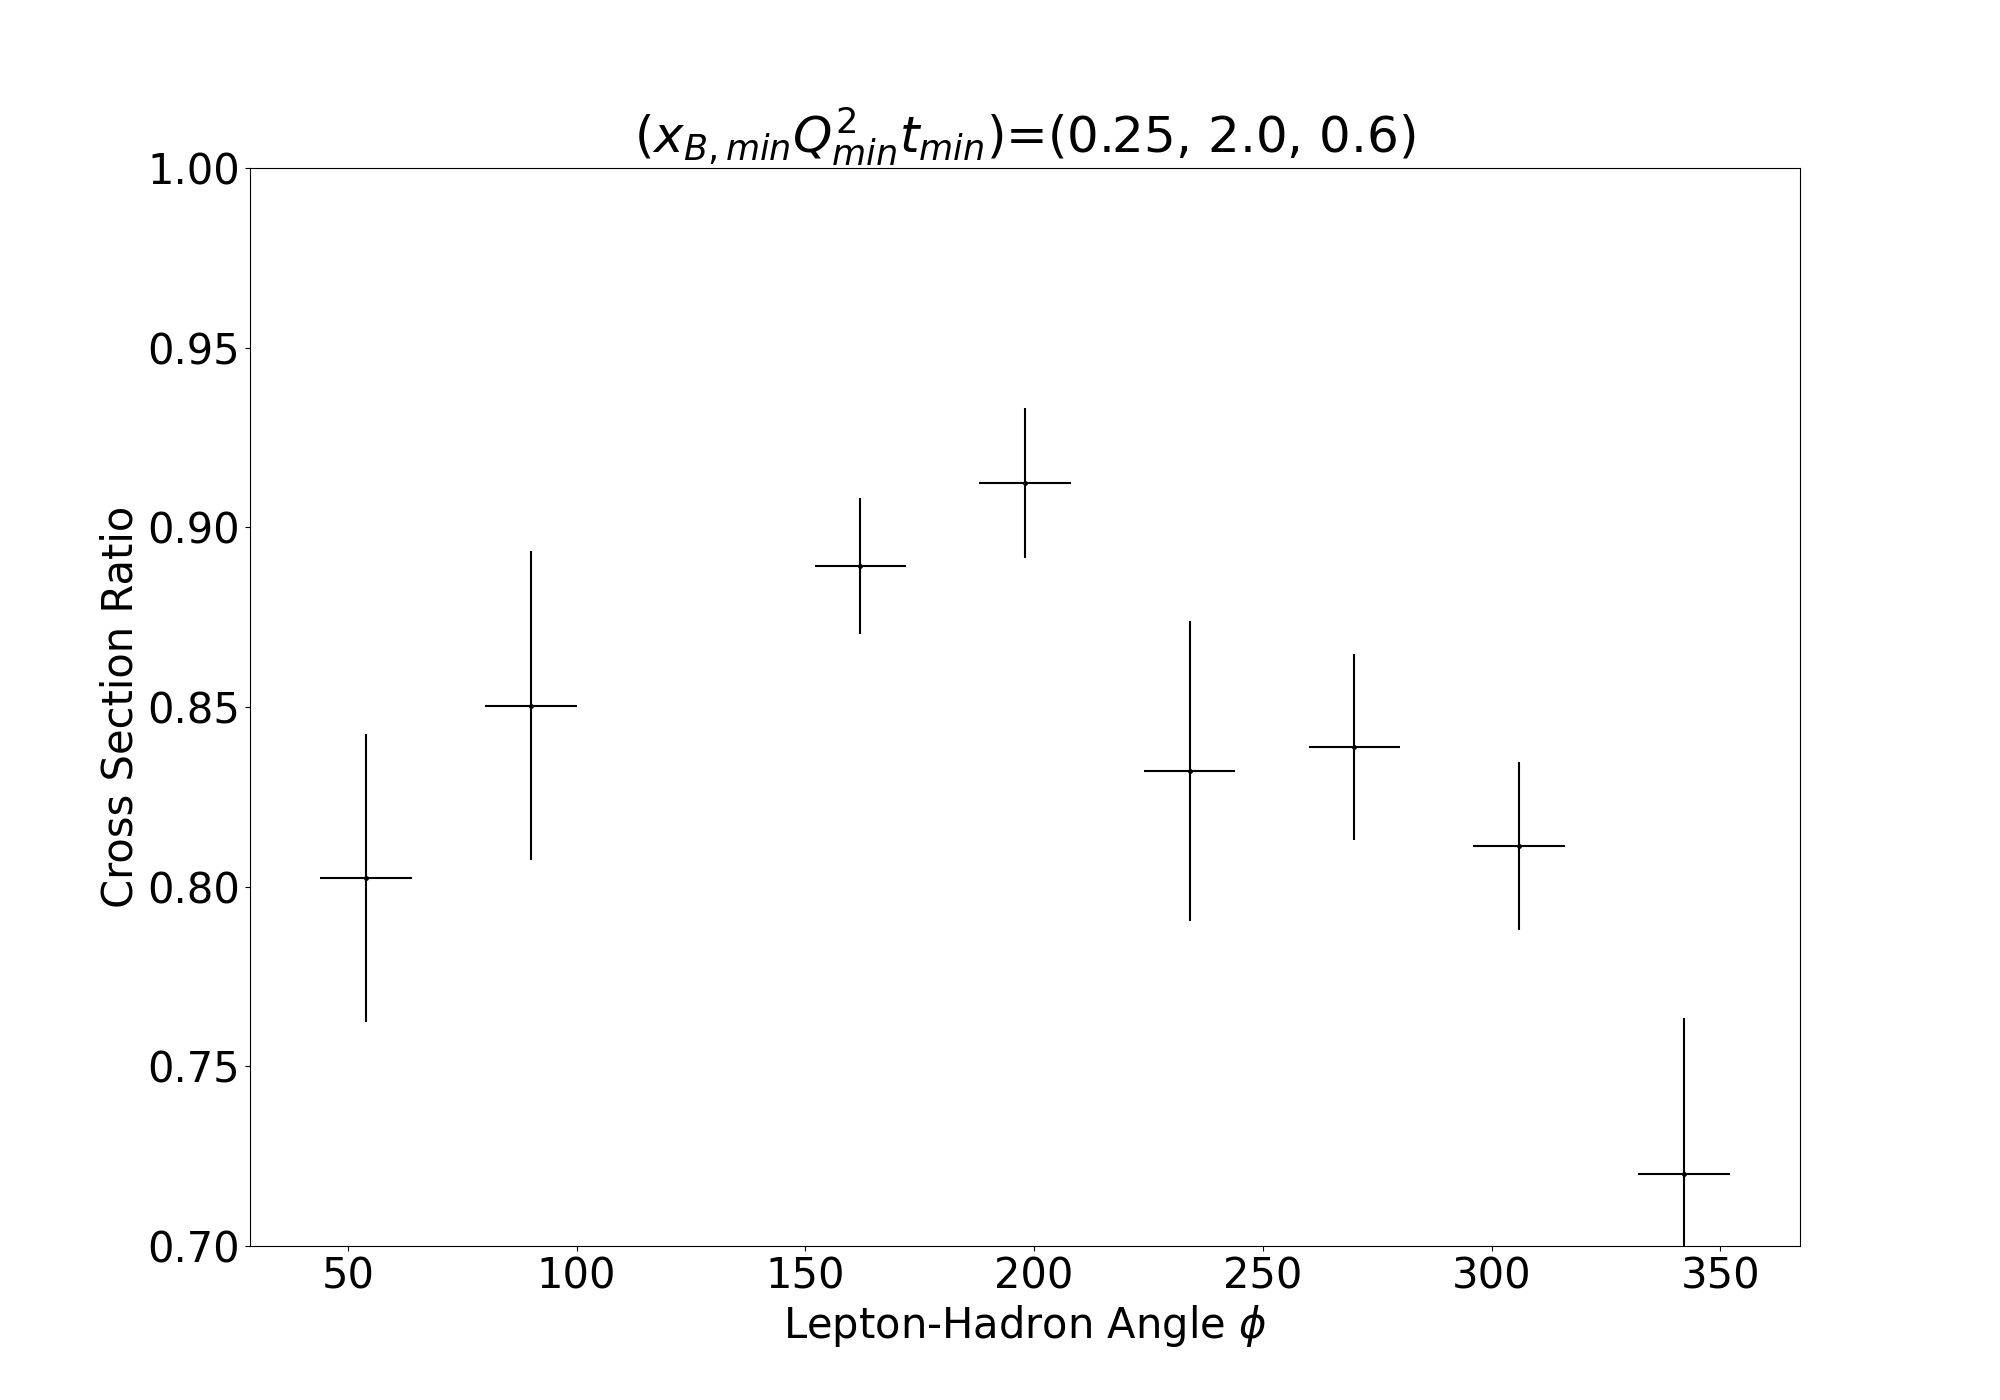
\includegraphics[width=0.5\textwidth]{Chapters/Ch4-BaseAnalysis/4_Correction_Factors/A3_b_radiative_correction/xqt=(0.25, 2.0, 0.6).png}}

    \caption[Sample of Radiative Corrections ]{Radiative corrections factor for select bins.}\label{fig:radcorr}
    %\caption[Reduced Cross Sections Across $\phi$]{Reduced Cross Sections Across $\phi$}
\end{figure}

    \subsubsection*{Reconstruction Efficiency}

    Similar to radiative corrections, uncertainties in reconstruction were estimated by running simulations at different levels of current background merging (40nA, 45nA, and 55nA) and compared to the nominal 50nA datafiles. Differences were taken as a measure of systematic uncertainty. 

    \subsection*{Momentum Corrections, Smearing, and Exclusivity Cut Uncertainties}
    Uncertainties were generated for momentum corrections, smearing factors, and event selection by altering the momentum corrections and smearing factors by \pm 10\% and rerunning the analysis, and for exclusivity cuts by changing the thresholds to 2$\sigma$ (narrow) and 4$\sigma$ (wide). The differences in the resulting cross section values were taken as an estimate of uncertainty. 
        
    \subsubsection*{Overall Normalization}

    Absolute normalization remains an ongoing effort by dedicated working groups in the CLAS collaboration. At present, we can compare the CLAS12 data to the published CLAS6 result, which contains a large number of overlapping kinematic bins. By adjusting the virtual photon flux factor and epsilon terms for the higher beam energy, we can obtain a direct comparison between the work of \parencite{Bedlinskiy2014ExclusiveCLAS} and our efforts. Published values for the reduced cross sections from the CLAS6 experiment for the DV$\pi^0$P channel are available \href{https://journals.aps.org/prc/supplemental/10.1103/PhysRevC.90.025205}{here}. Overall, there is not a large systematic shift in either direction between the CLAS12 and CLAS6 values (observe \ref{fig:combined_t0.2}-\ref{fig:combined_t1.5}). Instead, we take the difference between the two sets of data points as a measure of systematic uncertainty. This uncertainty will be removed once the current absolute normalization is validated. 

    

    \iffalse
    No systematic shift observed between clas6 and clas12 results, although the bins had a descrpancy that is for now included as an error untilt he absolute normazliation is better undersoot by the collaboration. The pictures only show some of it. 

    The accepted results from the CLAS6 experiment  can be used as a cross check for this work. 

    \fi

\iffalse
\subsection{Uncertainty Summary}

    Below shows a table representing sample uncertainties for a typical bin. 

    \begin{table}[ht]
    \centering
    \begin{tabular}{|l|r|}
    \hline
    \textbf{Sources} & \textbf{Typical Scale (\%)} \\
    \hline
    \textcolor{red}{SAMPLE TALBE ONLY } & NOT REAL VALUES YET \\
    Event selection — exclusivity & 11.8 \\
    Event selection — PID & 12.9 \\
    Resolution matching & 8.8 \\
    Acceptance corrections & 9.3 \\
    Background estimation & 12.8 \\
    Normalization & 10.0 \\
    Radiative Correction & 3.5 \\
    Finite bin width effect & 3.6 \\
    Reconstruction efficiency & 4.0 \\
    \hline
    \textbf{Total} & 27.0 \\
    \hline
    \end{tabular}
    \caption{Typical Scale for Different Sources}
    \label{table:example_stats}
    \end{table}

\fi
    \iffalse

    $N_rec_55/N_rec_50$ / $N_rec_50/N_rec_50$
    $N_rec_45/N_rec_50$ / $N_rec_50/N_rec_50$
    take average

    $N_rec_rad/N_rec_norad$ / $N_rec_norad/N_rec_norad$ bin by bin

    add 10\% or whatever it is norm for absolute - figure out some ratio, overall systematic shift, and then include sangbaeks note about what is wrong with it

    infold acc-corr estiamtion

    Include 30\% uncertainties for 1,2,3 uncerts

    FINIT BIN

    The advantage of finer binning is to provide improved density estimation. The
acceptance corrections and the finite bin width effects should increase with the bin
size. However, the bin size cannot be narrower than the effective resolutions in the
binning variables to minimize bin migration. Extremely small bins would not have
any statistical significance in each bin, which would lead to an invalid analysis. It is
important to determine the optimal binning.nm566+[



]
    

    The asymmetry in the phi sensititivy is expected. 
    
    
    \subsubsection*{Bin Volume Corrections}
        The bin volume is not always kinematically full, for example the a large number of bins are kinmeatically restricted, no number of ecvents could ever be found. SO, the bin shape is changed / adjusted for particularly empty bins.


    
    \subsubsection*{Overall Normalization Corrections}
        Compare to CLAS 6
        Overall normalization currently estimated by comparing to CLAS6 results, where there is overlap
    \fi

